%!TEX root = ../dissertation.tex
\section{Methods} \label{sec:discussion:methods}

\subsection{Transcriptional Interactions: \emph{miRNeo}} \label{sec:discussion:mirneo}
The comprehensive (however justified this term may be) analysis of transcriptional interactions seems to be, for the moment, a rather marginal endeavour. At the beginning of my work on this dissertation, a database such as \emph{miRNeo}, even in its most basic form, was not available. Recently, some efforts have been published,\cite{Fan2016, Tokar2018} including one which has necessitated a name change of my database, which was previously called \emph{miRNet}.\cite{Lobentanzer2019a, Fan2016} The premise of the approach is simple: for a biological network that is structured in the way of interaction partners connected by molecular interactions, build a database that models interaction partners as nodes of a network, and their interactions as its edges (see Chapter 2). The technical implementations, however, diverge.

\emph{miRNeo} follows the philosophy of modelling the studied networks as closely as possible in the raw database, to keep data recall at a minimum in terms of storage and processing power requirements. Neo4j seemed like a fitting platform for its implementation, since it is focused around building large networks with flexible computational requirements and possesses an infrastructure for process optimisation. Additionally, it can be integrated into development environments common in bioinformatics, such as Java and R. Most of the work presented in this dissertation has been performed on Neo4j version 3.0, however, the release of Neo4j version 4.0 was just announced and promises to bring further improvement in terms of handling and performance.\cite{Neo4j2020}

The main drawback of graph database integration into biological applications is the difference in infrastructure to virtually all other data, which is in tabular format. The effort of transitioning data into a dedicated graph format is not justified for simple questions, such as the gene targets of a single miRNA. The practical creation of \emph{miRNeo} from raw data in its current extent, without accounting for development time, would take up the majority of a month in computational time on a standard 16-core personal computer. However, nested analyses with multiple levels, and dynamic analyses with multiple steps in which the analysis in the next step depends on the result of the previous, necessitate computationally efficient implementation, and \emph{miRNeo} was able to handle all complex questions that presented themselves during my work. The most computationally demanding questions were the comprehensive whole-genome feedforward loop analyses (Section \ref{sec:stroke:ffl}), which nevertheless were completed in a matter of hours.

The most important limitation of \emph{miRNeo} is the sum of limitations that apply to the raw data \emph{miRNeo} is created from. Small RNA targeting is immensely complex, and small RNA expression is even more tissue-specific than transcription factor expression.\cite{Nowakowski2018} Thus, all results from predictions, be they based on complementarity, evolutionary conservation, or physical modelling, and even experimentally validated interactions can currently not be seen as certain indications of an actual interaction in different contexts, making validations indispensable. However, complex multi-layer interactions are nearly impossible to validate, making this area of research highly dependent on inferral from circumstantial evidence. In 2017, Kenneth Kosik introduced an experimental model of miRNA interactions at a conference for non-coding RNA in neurodegenerative disease.\cite{Kosik2017p} The study included the successive knockout of each one of a set of 11 miRNAs and observation of the cellular phenotype for each of the resulting cultures in a high throughput setting; he gave the cost of these experiments to be in the million dollar range. According to Kosik, the knockout of \emph{each one} of the 11 miRNAs led to a loss of the particular phenotype, which implied that all 11 cooperated to govern the molecular basis of the phenotype. However, this kind of experimentation cannot be applied to all open questions simply for economical reasons, and additionally, there still has been no publication of the study in a peer-reviewed journal as of now (May, 2020).\cite{Kosik2020w}

Similarly, in transcription factor interactions, the shortcomings of raw data may transfer into the database. A very pertinent example of FANTOM5 misannotation is the controversy around the promoters of \emph{CHAT} and \emph{SLC18A3} (see also Section \ref{sec:database:tf}). Since, by the statement of a FANTOM5 scientist, it is possible that the 5'-peaks of the two genes may have been confused because they lie in such close vicinity, it is not possible to distinguish between \emph{CHAT} and \emph{SLC18A3} in this data, or even state with certainty which of the two is implied in an analysis. However, as the immune cell data underlying Figure \ref{fig:tsne-large} shows, it is very feasible that the \emph{SLC18A3} signal in reality refers to \emph{CHAT} expression, because blood-borne immune cells do not require a vesicular transporter, but have been proven to express \emph{CHAT}. An advantage in modelling transcription factor interactions, however, is that in using FANTOM5 data and secondary sources such as Marbach \emph{et al.}\cite{Marbach2016} we are one step further than we are in small RNA analyses: we can differentiate between interactions in the different cell types of the human body. In extension, we can also infer on small RNA regulation in a cell type-specific manner by applying our knowledge on transcription factor interactions in these cell types, as we have attempted in the analysis of blood cell-specific networks in stroke (Section \ref{sec:stroke:celltypes}).

But even simpler shortcomings of the raw data in \emph{miRNeo} must be acknowledged: for instance, the annotation of biologically active molecules, be it DNA, RNA, or proteins, is always in flux, which together with the multiple institutions handling annotation leads to foreseeable deficits in translation between one set of data to the other. Particularly in whole-genome analyses (or likewise whole-miRnome etc.), individual control of every nomenclature deficit that results in loss of information (e.g., gene identifiers are different in experimental data and database) is not possible. For this reason, I integrated several identifiers (e.g. Entrez, HGNC, ENSEMBL) with failsafe mechanisms for the identification of as many molecules as possible. Still, there has been loss in several of the analyses. For miRNAs, the newer version 22 of miRBase annotation has not yet been implemented, since it may have caused compatibility issues with previous results.

Consequently, the more complex assessments suffer from a combination of single shortcomings of the raw data. For instance, feedforward loops are only feasible in a very particular constellation (see also Section \ref{sec:stroke:ffl}): because we lack information on TF$\to$smRNA interactions, smRNA species have to be at the center of the loop (\emph{X}), and transcription factors have to assume the role of controlling while being controlled (\emph{Y}). Associations of the kind TF$\to$smRNA are still in the stage of anecdotal evidence, for instance the HDAC7/RARA/miR-10a circuit (Figure \ref{fig:mir10-circuit}).\cite{Lee2017}

\begin{figure}
\centering
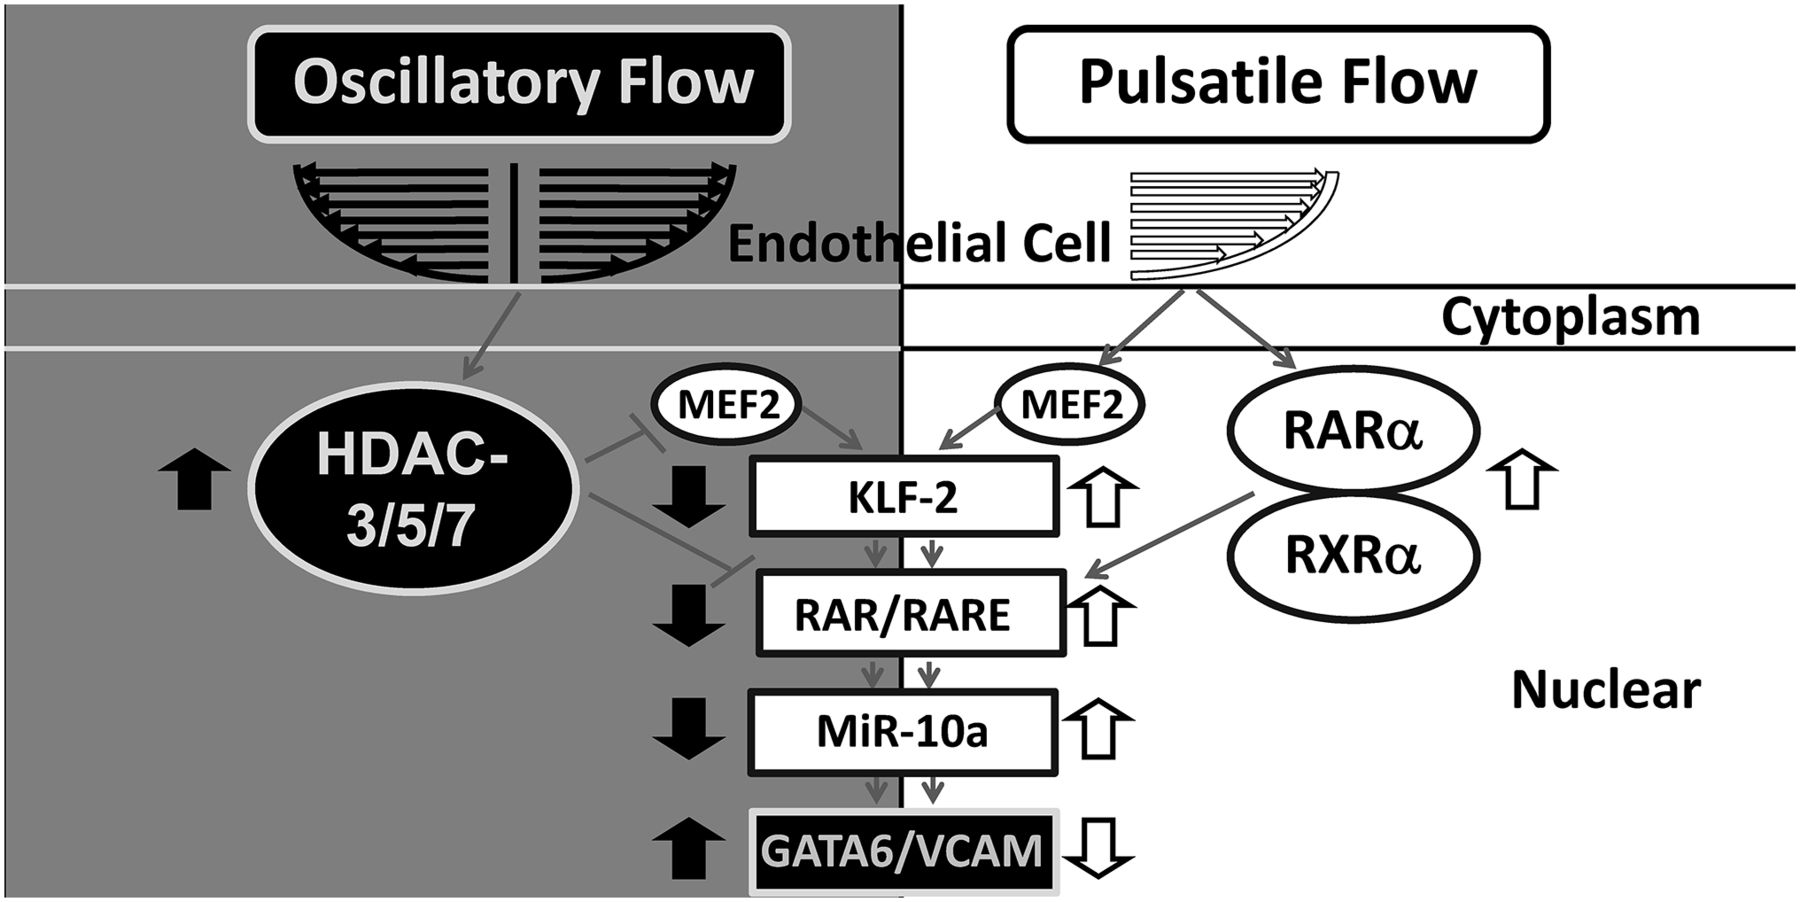
\includegraphics[width=.7\textwidth]{figures/mir10-circuit}
\caption[HDAC7/RARA/miR-10a Circuit.]{\textbf{Schematic diagram of the roles of hormone receptors and HDACs in modulating miR-10a expression and hence proatherogenic and antiatherogenic signaling in EC in response to different flow conditions.} Boxes with black and white shading represent proatherogenic and atheroprotective molecules, respectively. Image and caption from Lee \emph{et al.}\cite{Lee2017}
\label{fig:mir10-circuit}}
\end{figure}

\subsection{RNA Sequencing} \label{sec:discussion:rna-seq}
By 2020, \ac{seq} has by and large outgrown the teething troubles of its initial technological phase. However, the method itself brings with it inherent, largely mathematical problems. A lack of reproducibility was a great concern in the initial periods of RNA-seq, but the reproducibility of cholinergic cell culture (Section \ref{sec:cellculture:sequencing}) as well as the validations performed on small RNA during the studies of stroke patient blood (data not shown in this dissertation, but in the associated publication\cite{Winek2020}) show an agreeable reliability of the method in our hands.

Unrelatedly, the multiple testing problem still remains a pertinent issue of modern molecular biology. It is now more impressive to find a negative result in one of these analyses (e.g., no differential expression in a reasonably powered sequencing experiment) than it is to find actual differences. The question of where to place the threshold of significance, or whether to use such a threshold at all, is still a matter of very lively debate among scientists of many disciplines; additionally, consensus thresholds vary between fields or even between different kinds of assay. This dissertation, in general, follows the philosophy of balance between limiting false positives (by monitoring false discovery rate and utilising cross-experimental comparison) and identifying »real« changes (by monitoring adequate powering and effect sizes). In the limited area of RNA-seq, this is still manageable, because standard approaches in the form of multiple correction for differential expression analysis (e.g. in DESeq2,\cite{Love2014} which essentially uses Benjamini-Hochberg correction) and power analysis packages (I used R/powsimR\cite{Vieth2017}) already exist; in the extended graph-based network analyses, the matter is more complicated (see below in Section \ref{sec:discussion:network-statistics}).

For sequencing, particularly of small RNA, there remain open questions about the nature of detection. For instance, the alignment from raw sequencing reads of the two different smRNA species surveyed in Chapter 4 is handled by two separate software solutions, each tailored exactly to the biological nature of the respective smRNA species. I used miRExpress, version 2,\cite{Wang2009} to align miRNA sequences, and MINTmap\cite{Loher2017} for the tRNA fragments (more specifically, only the fragments »exclusive to the tRNA space«). Procedurally, there is no argument or consensus against analysing these two species separately, and unifying results afterwards. The main effect of concatenation of the two count tables for joint analysis in DESeq2 differential expression analysis is a loss in sensitivity, because multiple testing has to be corrected in relation to the number of unique analytes. However, since the hypotheses assumed before analysis included modes of cooperation between the two distinct species, I decided to test them together rather than apart from each other. The inspection of MA plots (see e.g. Figure \ref{fig:apeglm-comp-la2d4}), effect size distribution, and the comparison to separate analyses for both species all indicated the joint approach to be feasible. The loss in specificity was mild in miRNAs, joint analysis reproduced 98.4\% of detected and 83\% of differentially expressed miRNAs (FDR < 0.05), and 98.3\% of differentially expressed miRNAs with high effect size (absolute \ac{lfc} > 1.4). For tRFs, the loss was greater; joint analysis reproduced 96.1\% of detected, but only 20.5\% of differentially expressed tRFs. This can be explained by a high number of very lowly expressed tRFs compared to miRNAs: tRFs with high differential expression effect size (\ac{lfc} > 1.4) were reproduced at 52.1\%; and reproduction in the top 5 percentile by count-change was 92.3\%. Notably, this 95th percentile count-change cutoff value is at an absolute count-change of 28.5, meaning the loss of differentially expressed tRFs compared to separate analysis happened in the very low expression range, which is more desirable than it is a problem. An alternative solution would have been the truncation of low-count analytes before differential expression analysis; however, the threshold for such a step is always arbitrary, and thus truncation is no longer recommended.\cite{Zhu2019}

\subsection{Statistical Analyses of Network Interactions} \label{sec:discussion:network-statistics}
There is much less consensus when it comes to statistical interpretation of network analyses. This may in part be a result of network analyses being relatively uncommon compared to, for instance, sequencing experiments, and thus a lack of community consensus on how to approach certain problems. Often, a »network analysis« is a very confined, ultimate visualisation of the impact of one or few miRNAs with several genes that seem pertinent to the publication (for an example see Figure \ref{fig:example-network}). Thus, there is often no need to characterise the statistical relevance of the shown relationships, as they serve as a visualisation of hypotheses, or an illustration of a proposed pathway. In contrast, most network analyses presented in this dissertation are intermediary steps, the results of which are supposed to aid in identification of pertinent factors in the molecular interactions studied. As a result, there is a need to measure the relevance of each component of the network, as well as the validity of its message as a whole. Those can be approached in different ways, as is described in the following.

\begin{figure}
\centering
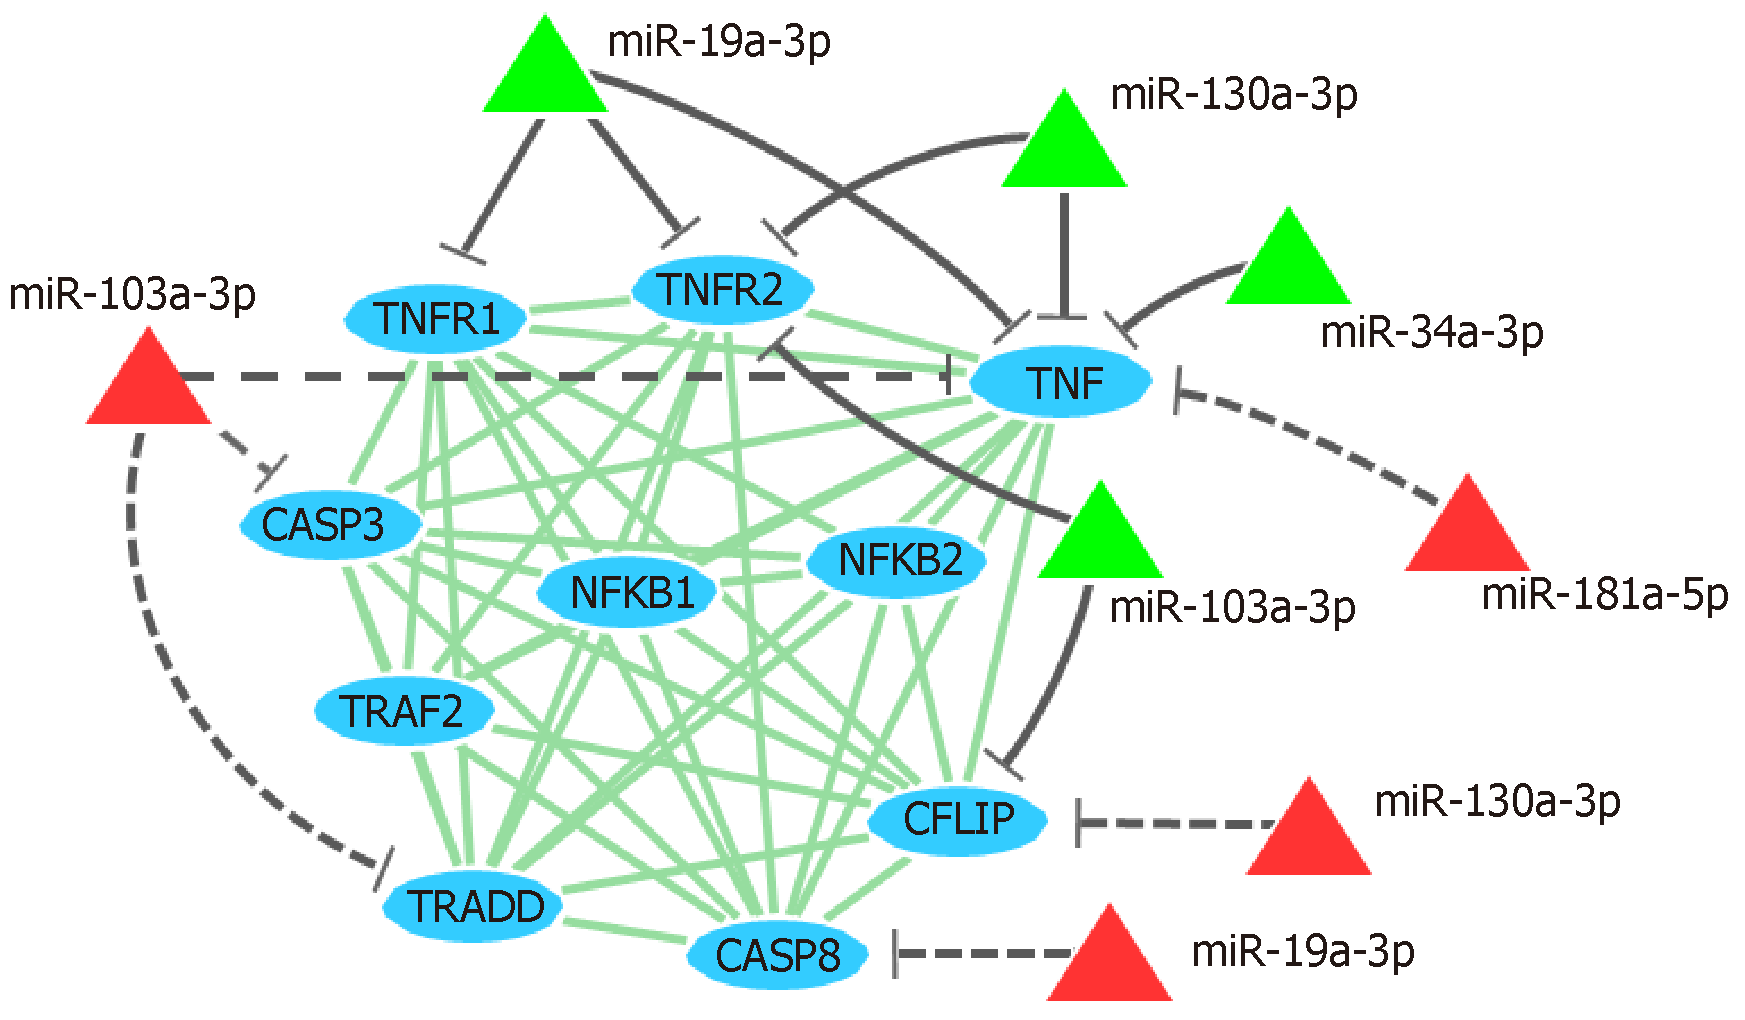
\includegraphics[width=.6\textwidth]{figures/example-network}
\caption[miRNA-Interaction Network Example.]{\textbf{Interaction network showing miRNAs and their predicted and validated targets.} The protein interaction network (light gray lines) shows the interaction between proteins (ellipses) encoded by tumor necrosis factor-$\upalpha$ pathway genes. Green triangles and solid gray lines represent miRNAs and validated target genes, respectively; red triangles and dotted gray lines represent predicted relationship between miRNA and target genes, respectively. TNF: Tumor necrosis factor. Image and caption from Rossi \emph{et al.}\cite{Rossi2019}
\label{fig:example-network}}
\end{figure}

The validity of single network components is subject to various pre-existing properties. To make this discussion more tangible, I will give an example of the most common single component in my analyses: a miRNA$\to$gene interaction. A first measure of its validity can be the existence of a validation experiment of this interaction. This is reflected in the scoring inside the database. The limitations as discussed in Section \ref{sec:discussion:mirneo}, e.g. in regard to tissue specificity, still apply. Below this highest level of stringency are the predicted interactions. As has been discussed previously by others, miRNA$\to$gene relationship predictions are best seen in comparison to other models, and most valuable predictions are the ones that several prediction algorithms agree upon, particularly if these algorithms are based on modelling different aspects of miRNA$\to$gene binding.\cite{Witkos2011} For this reason, I implemented the largest collection of algorithms I could find at the time (miRWalk 2.0\cite{Dweep2015}), supplemented by other sources as they became available, and also statistically evaluated the performance of all included algorithms to select a suitable subset for the summation of scores (Section \ref{sec:database:mirna}). These steps were undertaken to minimise the risk of bias by using as many sources as possible, while still retaining an amount of flexibility in analysis. For instance, if the resulting gene network was too large for sensible analysis, its size could be easily decreased by elevation of the score threshold, thus making the analysis more stringent.

The scoring threshold as used for miRNA interactions is not available for tRFs, because there are no prediction datasets available yet. The prediction was performed in-house on miRNA-like seeds of each detected differentially expressed tRF, which brings two important limitations: it assumes a miRNA-like functionality of tRFs, disregarding other interaction principles that have been found (see Section \ref{sec:intro:trfs}); and it limits the prediction sources to one, TargetScan.\cite{Friedman2009} TargetScan was selected for its approach of measuring evolutionary conservation of putative target sites, a measure that is very valuable in the case of tRFs, because we know little about any other parameters that could be relevant for the targeting. Since tRNAs and their fragments have been part of mammalian cells for a long time, evolutionary conservation of target sites in the genetically flexible 3' UTRs is a significant measure of functionality.\cite{Agarwal2015} Thus, for tRFs, the aggregation score of multiple algorithms was substituted with the conservation score generated by branch length (BL) and probability of conserved targeting (P$_{CT}$).\cite{Agarwal2015}

However, these cautionary steps still cannot preclude any and all possible biases that may be inherent to prediction models, and thus, statistical analyses on the basis of this general procedure are desirable. The simplest, most practical, although computationally intensive solution to inherent database biases is permutation (see Section \ref{sec:database:permutation}). Briefly, a null distribution of the measured parameter (e.g., miRNA$\to$gene interaction score) is generated by iterative analysis of randomly permuted datasets of the same size as the »real« dataset to be tested. The location of the »real« score inside this null distribution then gives the »extremity« of that real result, and thus the likelihood of the result being as extreme by chance, which equals \acf{fdr}. However, this approach requires a defined set of analytes that present with a measurable attribute (e.g., multiple miRNAs targeting one gene, or a defined set of target genes for any one miRNA). An additional measure to ensure robustness of this approach is the iteration across a range of parameters, for instance, a sliding score cutoff. Results staying »significant« across a range of different cutoffs may be an indication of their robustness. However, for each level of iterations added, computation time also increases. Since permutation approaches usually require tens to hundreds of thousands of iterations, the computational requirements can be considerable.

The advantage of permutations, as opposed to the disadvantage of having to test a set of multiple entries, is its scalability. Thus, permutations can also be used to assess the validity of the entire network, for instance by random permutation of case-control status (applicable in patient scenarios, as in Chapter 4), or of another attribute (such as sex, as in Chapter 3).

\subsection{Cholinergic Cellular Models: LA-N-2 and LA-N-5}
The decision to use a human cellular model of cholinergic neuronal cells was driven by two main factors: I) \emph{In vivo} experimentation, i.e., animal-based research, is not reliable as a model of complex human neuropsychiatric diseases.\cite{Nestler2010, Drummond2017, Sommer2017} II) Particular to RNA-based mechanisms, the difference between rodent and human genes is enormous, for instance in 3' UTRs that are not subject to the same evolutionary pressure as coding regions, which leads to low transferability of the application of hypothetical therapeutic oligonucleotides.\cite{Mor2013} Furthermore, so-called »3D cell cultures« or co-cultures of human cells of different types (e.g., neurons with astrocytes) are still not as developed as is necessary for stable experimentation, particularly in the case of cholinergic systems;\cite{Watson2017} thus, we opted for mono-culture of neuronal cell lines. Even in traditionally cholinergic research, the number of human neuronal models representative of actual cholinergic neurons is very low; the popular cell line SH-SY5Y had to be excluded after in-depth experimentation because it fails to express sensible amounts of the main cholinergic marker \emph{CHAT} and the vesicular transporter \emph{SLC18A3} even upon differentiation.\cite{Korecka2013}

LA-N cells were the logical alternative in the search for an adequate cholinergic model, although their maintenance is not as straightforward as that of many of the work-horses of human cell culture. The main argument for their selection was their natural expression of \emph{CHAT} and \emph{SLC18A3} as well as an impressive induction of these genes via stimulation by neurokines. This expression of \emph{CHAT} is a pivotal factor in the studies of cholinergic neurons, because there is much confusion about what constitutes a cholinergic cell in the CNS, and about the properties of the different cholinergic populations in the different brain regions. By definition, cholinergic neurons must be able to synthesise ACh (\emph{CHAT}) and release it through vesicles (\emph{SLC18A3}). Additionally, the high affinity choline uptake mediated by the SLC5A7 transporter is highly correlated with these two central markers in the nervous system (own results, Figure \ref{fig:chat-hacu-corr}, Yuliani \emph{et al.}\cite{Yuliani2020}). Other defining properties of cholinergic neurons are more optional (for instance, the defining property of basal forebrain cholinergic projection neurons to receive the retrograde NGF signal via \emph{NTRK1}). An additional benefit was the availability of LA-N cells of both sexes, which aided in studying sex differences in Lobentanzer \emph{et al.}\cite{Lobentanzer2019a}

\begin{figure}
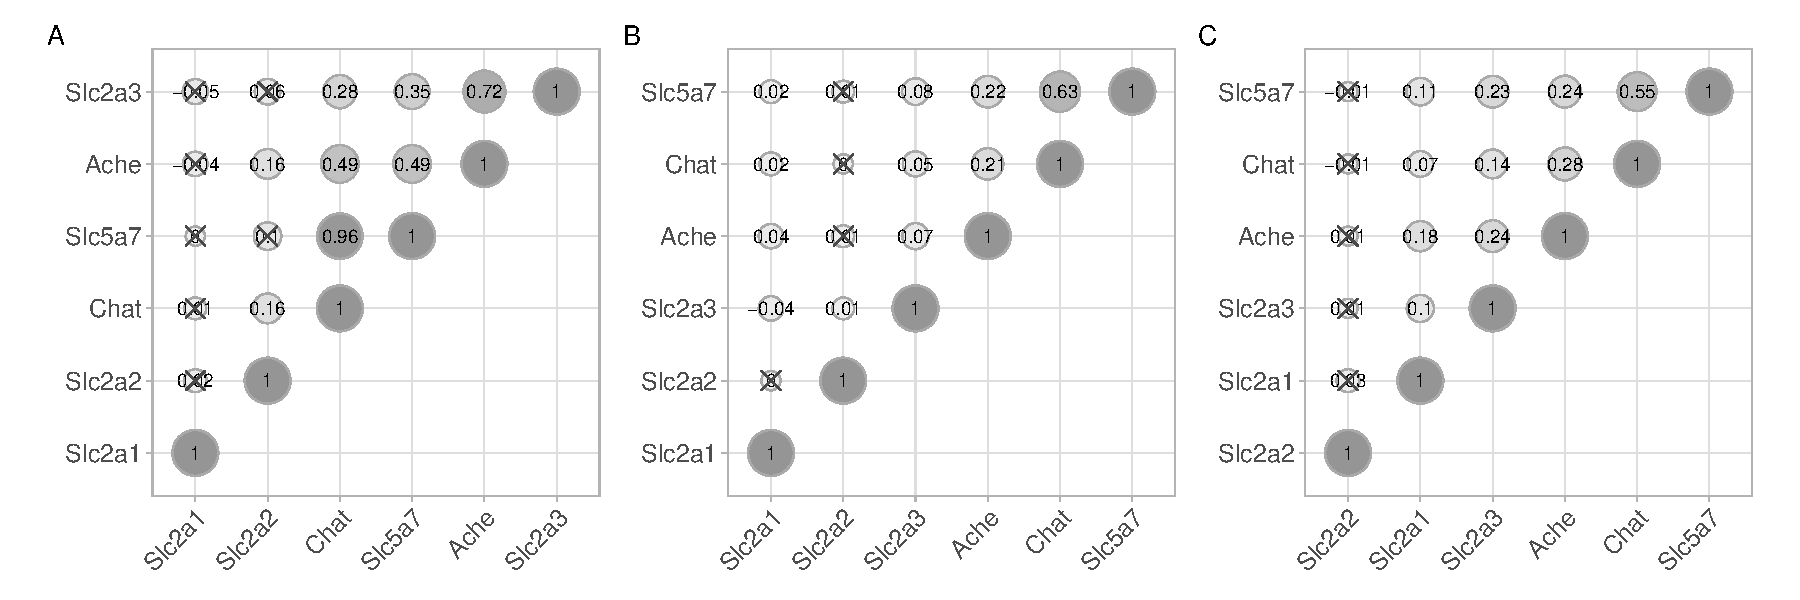
\includegraphics[width=\textwidth]{figures/chat-hacu-corr}
\caption[Correlation between CHAT and SLC5A7 in Nervous Cells.]{\textbf{Correlation between CHAT and SLC5A7 in Nervous Cells.} CHAT: choline acetyltransferase, SLC5A7: high affinity choline transporter (also known as CHT1), SLC2A1-3: passive glucose transporters. Size and depth of colour of circles denote strength of correlation (Pearson’s product-moment correlation coefficient, PPMCC), numbers denote PPMCC (range: -1 to 1). Non-significant correlation coefficients (p > 0.05) are crossed out. Rows and columns are ordered by hierarchical clustering, representing similarity of PPMCC values (Euclidian distance). (A) Correlation of transcripts in all tissues (cell-type-level) of the murine nervous system. (B) Correlation in all neurons (single-cell-level) of the murine nervous system. (C) Correlation in cholinergic neurons (single-cell-level) as determined by expression of the vesicular ACh-transporter, SLC18A3. Modified from Yuliani \emph{et al.}\cite{Yuliani2020}
\label{fig:chat-hacu-corr}}
\end{figure}

The decision for a mono-culture of immortalised human neuronal cells naturally introduced limitations common to all similar models: the cells are derived from tumour cells and do not resemble a physiological cell any more, otherwise they would not have lost senescence. All biological implications derived from these models have to be interpreted based on this central limitation. However, interpretation is based on the assumption that basic molecular processes, such as the control of mRNA by miRNAs, are still intact. Additionally, the cell communities generated \emph{in vitro} that are the basis of bulk sequencing analyses are very homogeneous, more so than any tissue derived from a living multi-cellular organism. While this enables bulk sequencing without »dilution« by supporting CNS-derived cells, as would be the case in patient brain region bulk sequencing, it also introduces a »non-natural« homogeneity in the RNA derived from the lysis of these cells and therefore harbours the danger of exacerbated sensitivity in differential expression. This may lead to the false positive identification of differentially expressed smRNAs, particularly those with a low base expression or small changes. However, controlling of effect sizes (e.g., a cutoff for absolute \acl{lfc}, or analysis of count-change) is well suited to prevent many irrelevant false positives.

\subsection{Stroke Patient Blood Samples} \label{sec:discussion:stroke-blood}
The main limitations in the sequencing of post-stroke patient blood are the lack in cell type specificity of RNA generation and the composition of the patient collective, which resulted in exclusion of females for balancing reasons and thus contains only male patients. Additionally, the controls by principle have to be external, since stroke is an unexpected event and thus there is virtually no possibility of attaining blood samples of patients pre-stroke except in very specific clinical conditions. As a result, control samples are healthy volunteers that have to be matched in a manner that reproduces the patient collective as closely as possible, which often cannot be more specific than matching for sex and age. Strictly speaking, the results of analyses based on the differential expression profile can only be applied to male patients. However, the tissue-specific analyses performed on small RNAs as well as on transcription factor interactions are based on large data collections representative of many male and female volunteers, and thus the CD14$^+$-related analyses, such as the \acl{ffl} analysis in Section \ref{sec:stroke:ffl-cd14}, can in large parts be applied to both sexes.

Section \ref{sec:stroke:celltypes} exclusively deals with the shortcomings of sequencing whole blood instead of isolated cellular components. Whether this method of extrapolation serves the purpose of explaining the roles of the tissues involved in smRNA stroke response remains to be clarified. However, translational approaches such as the one presented in Section \ref{sec:stroke:celltypes} can also aid in studying the transferability of whole blood results (which may be more common in the clinical setting) to tissue-specific analyses, which often require complex and costly purification steps in acquiring the isolated cell populations.

\subsection{Gene Ontology Analyses} \label{sec:discussion:go}
Some of the approaches to dimensionality reduction presented here rely heavily on the analysis of enrichment of genes in ontological categories of biological processes. The primary purpose of using GO enrichment as a tool is to deal with the reality of not being able to know all functions of any given gene. Strictly speaking, here also apply the same limitations as to other datasets of curated information: the quality of results depends on the quality of annotation in the raw ontology collection. For some lesser known proteins, these annotations may well be far from complete, and thus, the interpreting scientist is in danger of presentation bias. Similarly, by interpreting the list of ontological terms yielded by an analysis, terms may be selected or discarded based on their perceived relevance to the topic of study; inadequate knowledge about all participating processes may lead to the dismissal of relevant terms, constituting confirmation bias. To try and avoid large amounts of this form of confirmation bias, GO terms were presented in comprehensive form or as curated selection of all available data as much as possible (see for instance Figure \ref{fig:mir-de-fam-go}\,B and Section \ref{sec:stroke:ffl-cd14}). Additionally, the visual display of GO terms as a t-SNE projection, where distance is based on the amount of shared genes between the terms (using R/gsoap\cite{Tokar2020}), can aid in identifying the underlying categories of processes and their relationships to one another. This is further supported by the weighing functionality of R/topGO analysis,\cite{Alexa2006} whereby less specific parent GO terms are dismissed in favour of the more specific child nodes in the DAG graph (see also Sections \ref{sec:database:gsea} and \ref{sec:cellculture:topgo}).

An intriguing possibility is the transfer of ontology analyses of smRNA-targeted protein-coding transcripts to facilitate an understanding of the biological processes controlled by the smRNA interference. The approach is still underdeveloped in several regards: I) The weighing of smRNA$\to$gene relationships has a large influence on the outcome, making iteration and testing of robustness indispensable. II) The resolution of annotation is much coarser than in direct gene annotation. Due to the many-to-many nature of the miRNA interactome, functional implications for any one miRNA strongly intersect with other, similar miRNAs. This is the main reason for the analysis of families instead of single miRNAs in Section \ref{sec:cellculture:topgo}. In summary, while the derivation of function of miRNAs from their targeted genes is tempting in the light of a complete lack of direct functional annotation for miRNAs, this projection approach will have to be developed and validated before it can be routinely applied.

\subsection{Feedforward Loop Analyses} \label{sec:discussion:ffl}
Feedforward loop analysis brings together most of the issues discussed above. I) It is based on the aggregation of several types of molecular targeting relationships and thus is subject to their individual limitations. II) It is applied to the results of differential expression in stroke patient blood, and thus is also influenced by sequencing-related issues. And III) The modules yielded by FFL stratification are then scrutinised with the help of GO analysis to find gene collectives relevant to stroke.

Regarding I); the results of concatenation of these individual relationship types are unknown and difficult to measure. Every kind of influence on the validity of results is imaginable: the insecurities from each individual method may be additive, or even super-additive, making the end result more unreliable in consequence. Alternatively, the processes being firmly rooted in the biological reality of the cell may also have a corrective function on the end result, effectively acting as a filter that removes »illogical« circuits from the output, thus increasing its validity. There is no measure for answering this question as of now. However, the circuits and their ontological associations gathered in Chapter 4 make sense from a biological perspective, and, maybe more importantly, they make more biological sense than an observation of only differentially expressed genes, or only of smRNAs. In short, although the evidence is circumstantial, the message gained from FFL analysis may be larger than the sum of its parts. A more detailed discussion of the individual findings is held in the individual module descriptions of Section \ref{sec:stroke:ffl-cd14} and Section \ref{sec:stroke:resolution}. The substantiation of FFL analyses and their biological meaning is an important topic for further research.

Regarding II); sequencing-related issues need to be primarily controlled in the process of differential expression analysis. During feedforward loop analysis, results from differential expression are fixed, and thus cannot cause much confounding if they are used in a descriptive way, as is the case in my analyses. Should they be used beyond that, for instance, to weigh targeting relationships by the differential expression of their participating factors, more care has to be taken that the model applied makes sense. Although the approach is feasible in principle, the practical application in FFL analysis is not trivial. Generally, it makes sense to compare the expression levels of smRNAs and their target genes, for two main reasons, as is detailed below.

One: In the cellular context, any interaction is only practically relevant if the expression levels or changes in expression are on the same scale for both smRNA and mRNA. Of note, the count-change measure introduced in Lobentanzer \emph{et al.}\cite{Lobentanzer2019a} is much more suited to this assessment than the commonly used \ac{lfc}, because the latter does not relate to expression levels at all. However, until the sequencing of small and large RNAs can be routinely done in the same experiment (i.e., on the same microfluidic chip), the comparison of base mean expression (or count-change) between small and large RNA will always be very approximate, because it is dependent on sequencing depth of the individual experiment. 

Two: Considering miRNA-like behaviour, those interactions will be particularly interesting where the smRNA is regulated inversely to the target mRNA. However, this concerns only the theoretical interaction of two isolated partners, whereas the smRNA$\to$gene interactions in live cells are layered and only the strongest single relationships will have a chance of prevailing against the regulatory »chaos« that is an actual cell. This alone precludes actual analysis of differential expression influence on smRNA targeting (apart from complex mathematical models which remain to be established), without even considering the third interaction partner, transcription factors. Those introduce another element of uncertainty: although we know more about their tissue specific activities through efforts such as Marbach \emph{et al.}\cite{Marbach2016}, we do not specifically know which transcription factor acts on a promoter or repressor towards which genes in which tissues. Mathematical structural models able to predict these interactions in a cellular, whole-genome context are desirable, but not yet a reality.

Regarding III); the main criticism of proceeding from comprehensive FFLs through modularisation to GO analysis is the arbitrary nature of network modularisation. Modularisation itself is a purely mathematical process of describing the interconnectedness of nodes in the network, implemented by Blondel \emph{et al.} (»Fast unfolding of communities in large networks«).\cite{Blondel2008} The choice of resolution that yielded five communities in my analysis thus was largely arbitrary, selected in a way that correlated module identity with the visual clusters created by force-directed organisation of the FFL network. However, since the main purpose of modularisation is a reduction in dimensionality that facilitates human understanding, every possible resolution that results in a manageable number of modules may be seen as »reasonable«. A standardisation of these procedures is nevertheless desirable and will be subject of further studies.

%\newpage
